%Version 3.1 December 2024
% See section 11 of the User Manual for version history
%
%%%%%%%%%%%%%%%%%%%%%%%%%%%%%%%%%%%%%%%%%%%%%%%%%%%%%%%%%%%%%%%%%%%%%%
%%                                                                 %%
%% Please do not use \input{...} to include other tex files.       %%
%% Submit your LaTeX manuscript as one .tex document.              %%
%%                                                                 %%
%% All additional figures and files should be attached             %%
%% separately and not embedded in the \TeX\ document itself.       %%
%%                                                                 %%
%%%%%%%%%%%%%%%%%%%%%%%%%%%%%%%%%%%%%%%%%%%%%%%%%%%%%%%%%%%%%%%%%%%%%

%%\documentclass[referee,sn-basic]{sn-jnl}% referee option is meant for double line spacing

%%=======================================================%%
%% to print line numbers in the margin use lineno option %%
%%=======================================================%%

%%\documentclass[lineno,pdflatex,sn-basic]{sn-jnl}% Basic Springer Nature Reference Style/Chemistry Reference Style

%%=========================================================================================%%
%% the documentclass is set to pdflatex as default. You can delete it if not appropriate.  %%
%%=========================================================================================%%

%%\documentclass[sn-basic]{sn-jnl}% Basic Springer Nature Reference Style/Chemistry Reference Style

%%Note: the following reference styles support Namedate and Numbered referencing. By default the style follows the most common style. To switch between the options you can add or remove “Numbered” in the optional parenthesis. 
%%The option is available for: sn-basic.bst, sn-chicago.bst%  
 
%%\documentclass[pdflatex,sn-nature]{sn-jnl}% Style for submissions to Nature Portfolio journals
%%\documentclass[pdflatex,sn-basic]{sn-jnl}% Basic Springer Nature Reference Style/Chemistry Reference Style
\documentclass[pdflatex,sn-mathphys-num]{sn-jnl}% Math and Physical Sciences Numbered Reference Style
%%\documentclass[pdflatex,sn-mathphys-ay]{sn-jnl}% Math and Physical Sciences Author Year Reference Style
%%\documentclass[pdflatex,sn-aps]{sn-jnl}% American Physical Society (APS) Reference Style
%%\documentclass[pdflatex,sn-vancouver-num]{sn-jnl}% Vancouver Numbered Reference Style
%%\documentclass[pdflatex,sn-vancouver-ay]{sn-jnl}% Vancouver Author Year Reference Style
%%\documentclass[pdflatex,sn-apa]{sn-jnl}% APA Reference Style
%%\documentclass[pdflatex,sn-chicago]{sn-jnl}% Chicago-based Humanities Reference Style

%%%% Standard Packages
%%<additional latex packages if required can be included here>

\usepackage{graphicx}%
\usepackage{multirow}%
\usepackage{amsmath,amssymb,amsfonts}%
\usepackage{amsthm}%
\usepackage{mathrsfs}%
\usepackage[title]{appendix}%
\usepackage{xcolor}%
\usepackage{textcomp}%
\usepackage{manyfoot}%
\usepackage{booktabs}%
\usepackage{algorithm}%
\usepackage{algorithmicx}%
\usepackage{algpseudocode}%
\usepackage{listings}%
\usepackage{wasysym}%
%%%%

%%%%%=============================================================================%%%%
%%%%  Remarks: This template is provided to aid authors with the preparation
%%%%  of original research articles intended for submission to journals published 
%%%%  by Springer Nature. The guidance has been prepared in partnership with 
%%%%  production teams to conform to Springer Nature technical requirements. 
%%%%  Editorial and presentation requirements differ among journal portfolios and 
%%%%  research disciplines. You may find sections in this template are irrelevant 
%%%%  to your work and are empowered to omit any such section if allowed by the 
%%%%  journal you intend to submit to. The submission guidelines and policies 
%%%%  of the journal take precedence. A detailed User Manual is available in the 
%%%%  template package for technical guidance.
%%%%%=============================================================================%%%%

%% as per the requirement new theorem styles can be included as shown below
\theoremstyle{thmstyleone}%
\newtheorem{theorem}{Theorem}%  meant for continuous numbers
%%\newtheorem{theorem}{Theorem}[section]% meant for sectionwise numbers
%% optional argument [theorem] produces theorem numbering sequence instead of independent numbers for Proposition
\newtheorem{proposition}[theorem]{Proposition}% 
%%\newtheorem{proposition}{Proposition}% to get separate numbers for theorem and proposition etc.

\theoremstyle{thmstyletwo}%
\newtheorem{example}{Example}%
\newtheorem{remark}{Remark}%

\theoremstyle{thmstylethree}%
\newtheorem{definition}{Definition}%

\raggedbottom
%%\unnumbered% uncomment this for unnumbered level heads

\begin{document}

\title[On The Gravitational Nature Of Time]{On The Gravitational Nature Of Time}

%%=============================================================%%
%% GivenName	-> \fnm{Joergen W.}
%% Particle	-> \spfx{van der} -> surname prefix
%% FamilyName	-> \sur{Ploeg}
%% Suffix	-> \sfx{IV}
%% \author*[1,2]{\fnm{Joergen W.} \spfx{van der} \sur{Ploeg} 
%%  \sfx{IV}}\email{iauthor@gmail.com}
%%=============================================================%%

\author*[1]{\fnm{Andrew} \sur{Mueller}}\email{AndrewMueller414@gmail.com}

\affil*[1]{\orgname{Independent Researcher}, \orgaddress{\city{Milwaukee}, \postcode{53219}, \state{WI}, \country{USA}}}


%%==================================%%
%% Sample for unstructured abstract %%
%%==================================%%

\abstract{We explore a modified set of coordinate transformations that describe time, cosmic inflation and gravitational acceleration as the same process as observed from different reference frames through an unwrapped Kaluza-Klein like geometry. We show that these transformations satisfy Lorentz invariance in a $4 + 0$ space-time with a radion scalar potential of $1$. From this mechanism an equation is derived trigonometrically for galactic orbital velocity, reproducing local observation with only baryonic mass. Through these coordinate transformations, a direct mechanism to the equivalence principle is derived yielding multiple functions producing our peculiar velocity and a secondary velocity, as well as a geometric justification for the discrepency between SNe and CMB relative velocity calculations. These modified coordinate transformations produce a classical notion of simultaneity and indicate a novel model of chronology which resolves multiple temporal pardoxes without the need for selective reference frame bias.}

%%================================%%
%% Sample for structured abstract %%
%%================================%%

% \abstract{\textbf{Purpose:} We explore a modified set of coordinate transformations that describe time, cosmic inflation and gravitational acceleration as the same process as observed from different reference frames through an unwrapped Kaluza-Klein like geometry. 

% \textbf{Methods:} The abstract serves both as a general introduction to the topic and as a brief, non-technical summary of the main results and their implications. The abstract must not include subheadings (unless expressly permitted in the journal's Instructions to Authors), equations or citations. As a guide the abstract should not exceed 200 words. Most journals do not set a hard limit however authors are advised to check the author instructions for the journal they are submitting to.

% \textbf{Results:} The derived coordinate transformations satisfy existing experimental validations of special relativity while providing a set of 4 equations yielding our peculiar velocity, a resolution to the SNe/CMB discrepency and an orbital velocity equation that matches observation with only visible mass. This model has yet to be unified with the generali

% \textbf{Conclusion:} The abstract serves both as a general introduction to the topic and as a brief, non-technical summary of the main results and their implications. The abstract must not include subheadings (unless expressly permitted in the journal's Instructions to Authors), equations or citations. As a guide the abstract should not exceed 200 words. Most journals do not set a hard limit however authors are advised to check the author instructions for the journal they are submitting to.}

\keywords{gravitation, time, relativity, inflation}

%%\pacs[JEL Classification]{D8, H51}

%%\pacs[MSC Classification]{35A01, 65L10, 65L12, 65L20, 65L70}

\maketitle

\section{Introduction}\label{sec1}

Albert Einstein was insistent on a static Universe during the period in which he wrote his specialized theory of relativity\cite{einstein1905electrodynamics, Einstein1917CosmologicalConsiderations, ORaifeartaigh2017EinsteinCosmology, Nussbaumer2014EinsteinStaticToExpanding}(SR). What is proposed here is largely a re-examination of the geometry of SR under the assumption that the $\mathbb{R}^{3}$ space between two arbitrary points elongates as time progresses.

This dilation is then bound to $\gamma$, giving a velocity dependent function for $\vec{g}$ and a magnitude that extends into a 4th spatial coordinate, $y$, similar in construction to an unwrapped Kaluza-Klein (KK) dimension\cite{Kaluza1921, Klein1926}. Through these coordinate transformations time, cosmic inflation and gravitational acceleration become the same process as observed from different reference frames in a space-time geometry where the 4th spatial KK dimension acts as a concurrent density axis.

This geometry gives an alternative model of concurrency and synchronicity as a classical notion of simultaneity is maintained by attributing the additional spatial separation to the 4th spatial dimension, $dy = v \tau \sqrt{\gamma^{2} - 1}$ as shown in figure \ref{fig_trig_diagram}. While maintaining classical simultaneity resolves numerous temporal paradoxes without the need for selective reference frame preference, it produces a concurrent axis that describes the ultra-dense state of the early Universe as being separated only by some $\Delta$ along this 4th spatial axis.


\begin{figure}[h]
\centering
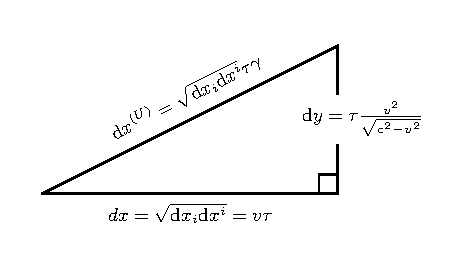
\includegraphics[width=0.9\textwidth]{./diagrams/outputs/simple_triangle.eps}
\caption{Right-triangle construction used to represent the ordinary spatial displacement $dx$, the additional spatial displacement $dy$, and the extended displacement $dx^{(U)}$. The relation assigned to the hypotenuse is an assumption of the proposed geometric construction.}\label{fig_simple_triangle}
\label{fig_trig_diagram}
\end{figure}



\subsection{The Lighthouse \& The Clock-Tower}

Let an event be defined classically, such that a single, instantaneous event represents a local measurement as $dt \to 0$.

Let there be two overlapping $\mathbb{R}^{3}$ coordinate systems, $\mathbf{S}$ and $\mathbf{U}$. Let $\mathbf{S}$ and $\mathbf{U}$ represent an equi-temporal surface within a 4-dimensional hyperspace where $y=y^{\left( S \right)}$ and $y=y^{\left( U \right)}$ in each respective 3-dimensional surface.

This gives

\begin{equation}
    f\left( x_{i}, y \right) = \partial_y \mathcal{H}
\end{equation}

where


\begin{equation}
    f\left( x_{i}, y^{\left( A \right)} \right) = \mathbf{A}\left( x_{i} \right)
\end{equation}

for an arbitrary $\mathbf{A}$ contained within $\mathcal{H}$.

Let $\mathbf{U}$ represent a `future' state from the perspective of an observer in $\mathbf{S}$ so that


\begin{equation}
    v^{\left( S \right)} = \left( t, x_{\mu} \right) \qquad v^{\left( U \right)} = \left( t + \Delta t, x_{\mu} \right)
\end{equation}

where $\Delta t > 0$ and $\mu = 1, 2, 3, 4$. Likewise, let $\mathbf{S}$ and $\mathbf{U}$ be bound such that 

\begin{equation}
    f\left( x_{i}, y^{\left( U \right)} \right) = f\left( x_{i}, y^{\left( S \right)} \right) + \int_{x_{0}^{\left( S \right)}}^{x_{0}^{\left( U \right)}} F\left( x \right)\ \mathrm{d}t
\end{equation}

where $F$ is the sum of all forces acting on the point of space at $x$, integrated according to time, which in turn sums the change between the temporal surfaces $\mathbf{S}$ and $\mathbf{U}$.

Let there also be two observers, $A$ and $B$. Let $A$ and $B$ agree that $B$ should travel at some \textit{agreed upon} relativistic velocity $v^{\prime}$ between two arbitrary points in space contained within $\mathcal{H}$, $p_{1}$ and $p_{2}$. Let the experiment be arranged such that $B$ passes $p_{1}$ in $\mathbf{S}$, and $p_{2}$ in $\mathbf{U}$.

Let $A$ remain at relative rest with respect to $p_{1}$, and at $p_{2}$ place a time keeping device large enough to be visible from $p_{1}$. 

We then make these assertions

\begin{enumerate}[1.]
\item To maintain a classical model of simultaneity $A$ and $B$ must agree upon the time at which $B$ reaches $p_{2}$.
\item To satisfy existing experimental evidence for the additional $\gamma$ factor\cite{Rossi1941, FrischSmith1963, Bailey1977, Bailey1979, Botermann2014}, $\Delta t = \gamma \frac{d}{v}$.
\end{enumerate}

This gives a set of coordinate transformations such that for each relative observer

\begin{equation}
    \Delta t = \overbrace{\frac{d \cdot \gamma}{v^{\left( U \right)}}}^{B} = \underbrace{\frac{d}{v^{\left( S \right)}} = \frac{d}{v^{\left( U \right)} \left( \frac{1}{\gamma} \right)}}_{A}
\end{equation}

\section{Theoretical Framework}\label{sec_theoretical_framework}

We acknowledge two primary properties of time:

\begin{enumerate}[1.]
\item A driving rate of change, at least as fundamental as the $\mathbb{R}^{3}$ dimensions.
\item A 4th displacement coordinate.
\end{enumerate}

Throughout the following derivations, we presume that time has no physical significance beyond the two properties described above. We presume that time acts only as a mathematical tool: $\Delta t = \frac{d}{v}$. In turn, we must attribute the 4th displacement coordinate to a position along the density axis that arises, $y$, and the driving rate of change to \textit{motion}.

Likewise, we presume that in a co-moving frame of reference along the $y$ axis, mechanical equations should limit at their Newtonian counterpart with only the relativistic portion of associated magnitudes protruding out of the containing temporal surface.


To remove time as a physically meaningful quantity, we let

\begin{equation}\label{eq_tau_definition}
\tau = \frac{\dot{x}}{\widehat{v}}
\end{equation}

where $\dot{x}$ indicates not a derivative with respect to time, but rather a fundamental driving rate of change, a magnitude of length that grows with an arbitrary temporal scalar. Let $\widehat{v} = \partial_\tau x\ \hat{\tau}$ where $\hat{\tau} = 1$, or the velocity in units of distance. $\tau$, while equivalent in magnitude to $t$ is derived directly from the geometry and has no explicit time dependence.


\subsection{Lorentz Invariance}

We consider these coordinate transformations with regards to the Lorentz transformations and find that for an instantaneous event where $dt \to 0$

\begin{equation}
\boxed{
\begin{gathered}
    dx' = \gamma dx = v^{\left( U \right)}\\
    c\,dt' = -\gamma\frac{v}{c}dx = - \partial_\tau y
\end{gathered}
}
\end{equation}

where $y$ is as defined in equation \ref{eq_dy_definition}.

We define $v \left( \gamma \right)$ to be the Lorentz factor solved for $v$

\begin{equation}\label{eq_v_of_gamma}
    v\left( \gamma \right) = c \sqrt{1 - \frac{1}{\gamma^{2}}}
\end{equation}

Beginning with the definition of the additional coordinate,

\begin{equation}\label{eq_dy_definition}
    y = \tau \frac{v^2}{\sqrt{c^2-v^2}}
\end{equation}

we take the partial derivative with respect to $\tau$, holding $v$ constant:

\begin{equation}
    \boxed{
    \partial_\tau y =
    \frac{v^2}{\sqrt{c^2-v^2}}
    }
\end{equation}

Since $x=v\tau$, we can equivalently express the coordinate
as a function of $x$:

\begin{equation}
    y = x\frac{v}{\sqrt{c^2-v^2}}.
\end{equation}

Taking the partial derivative with respect to $x$ gives

\begin{equation}
    \boxed{
    \partial_x y =
    \frac{v}{\sqrt{c^2-v^2}}
    }
\end{equation}

We can now express this derivative in terms of the Lorentz factor:

\begin{equation}
    \partial_x y =
    \frac{\gamma v}{c}.
\end{equation}

Multiplying by the velocity expressed as a function of $\gamma$,

\begin{equation}
\begin{aligned}
    v(\gamma)\partial_x y
    &=
    c\sqrt{1-\frac{1}{\gamma^2}}
    \frac{\gamma v}{c}
    \\[6pt]
    &=
    v\sqrt{\gamma^2-1}
    \\[6pt]
    &=
    \frac{\gamma v^2}{c}.
\end{aligned}
\end{equation}

Finall we recover

\begin{equation}
    \boxed{
    v(\gamma)\partial_x y
    =
    \frac{\gamma v^2}{c}
    =
    \partial_\tau y
    }
\end{equation}


\subsubsection{Invariance of the Minkowski Interval}

We can further examine the Lorentz invariance of these transformations by considering the Minkowski interval. For an instantaneous event, where $dt \to 0$, the transformed interval is given by

\begin{equation}
    ds'^2 = c^2dt'^2 - dx'^2.
\end{equation}

Substituting the coordinate transformations established above,

\begin{equation}
\begin{aligned}
    ds'^2
    &=
    \left(-\gamma\frac{v}{c}dx\right)^2
    -
    \left(\gamma dx\right)^2
    \\[6pt]
    &=
    \gamma^2 dx^2
    \left(\frac{v^2}{c^2}-1\right).
\end{aligned}
\end{equation}

Using the definition of the Lorentz factor,

\begin{equation}
    \gamma^2 =
    \frac{1}{1-\frac{v^2}{c^2}},
\end{equation}

we obtain

\begin{equation}
    ds'^2
    =
    -\gamma^2 dx^2
    \left(1-\frac{v^2}{c^2}\right).
\end{equation}

Therefore,

\begin{equation}
    \boxed{
    ds'^2=-dx^2=ds^2
    }
\end{equation}

Thus, the instantaneous coordinate transformations preserve the Minkowski interval, demonstrating consistency with the invariance condition of Lorentz transformations.

\subsubsection{The Lorentz Factor as a Coordinate Gradient}

Having established the relationship between the additional coordinate and the Lorentz transformations, we can rearrange the spatial derivative to express the Lorentz factor directly in terms of $\partial_x y$.

Recall that

\begin{equation}
    \partial_x y = \frac{\gamma v}{c}.
\end{equation}

Squaring both sides gives

\begin{equation}
    (\partial_x y)^2 = \frac{\gamma^2 v^2}{c^2}.
\end{equation}

Using the definition of the Lorentz factor,

\begin{equation}
    \gamma^2 = \frac{1}{1-\frac{v^2}{c^2}},
\end{equation}

we can rewrite this expression as

\begin{equation}
    (\partial_x y)^2
    =
    \frac{v^2}{c^2-v^2}.
\end{equation}

Rearranging and substituting back into the Lorentz factor gives

\begin{equation}
\begin{aligned}
    \gamma^2
    &=
    1+\frac{v^2}{c^2-v^2}
    \\[6pt]
    &=
    1+(\partial_x y)^2.
\end{aligned}
\end{equation}

Consequently, we obtain the following expression for the Lorentz factor in terms of the additional coordinate:

\begin{equation}
    \boxed{
        \gamma = \sqrt{1+(\partial_x y)^2}
    }
\end{equation}

This establishes a direct relationship between the Lorentz factor and the spatial gradient of the additional coordinate, allowing the relativistic factor to be expressed geometrically without explicitly introducing velocity.

\subsection{The Equivalence Principle}\label{sec_equivalence_principle}

Here we examine these coordinate transformations in the context of the equivalence principle. While a well defined function remains elusive, these generialized coordinate transformations and a numerical intersection with the fine structure constant allows us to derive several important properties of an apparent electromagnetic function producing $\vec{g}$.

\subsubsection{Earth's Kinematic Velocity From Electromagnetic Parameters}

We define $\delta\left( M, R \right)$ to be

\begin{equation}
    \delta\left( M, R \right) = \frac{d}{dR} g = 2 \frac{GM}{R^{3}}
\end{equation}

If $\delta\left( M, R \right)$ is induced by the coordinate transformations described above, we should presume that this dilation is radial. We then find the magnitude of a single $\mathbb{R}^{3}$ axis by taking the inverse of the determinant of a diagonal $3 \times 3$ matrix:

\begin{equation}
    \omega\left( M, R \right) = \sqrt[3]{\frac{d}{dR} g} = \left(\delta\left( M, R \right)\right)^{1/3}
\end{equation}


Investigating this quantity for Earth gives

\begin{equation}
    \omega_{\oplus} = 0.014537\dots
\end{equation}

While this approximates $2 \alpha$, it more closely produces

\begin{equation}\label{eq_omega_earth}
    \omega_{\oplus} = \alpha \left( 2 - \alpha \right) \pm 0.0253\%
\end{equation}

Then by expanding equation \ref{eq_omega_earth}

\begin{equation}\label{eq_omega_earth_Gamma}
    \alpha \left( 2 - \alpha \right) = \sqrt[3]{\frac{d}{dR}g}
\end{equation}

Moving the electromagnetic parameters and $R$ to one side before integrating with respect to $R$ gives


\begin{equation}
    R^{4} \left(\frac{e^{6} \left(\frac{\mu_{0}}{\epsilon_{0}}\right)^{\frac{3}{2}}}{4 h^{3}} + \frac{3 \mu_{0} e^{10} \left(\frac{\mu_{0}}{\epsilon_{0}}\right)^{\frac{3}{2}}}{64 \epsilon_{0} h^{5}} - \frac{3 \mu_{0}^{2} e^{8}}{16 \epsilon_{0}^{2} h^{4}} - \frac{\mu_{0}^{3} e^{12}}{256 \epsilon_{0}^{3} h^{6}}\right) = 1.272 \times 10^{21}
\end{equation}

We then take the radius independent magnitude, isolating the additional electromagnetic parameters

\begin{equation}
    \frac{e^{6} \left(\frac{\mu_{0}}{\epsilon_{0}}\right)^{\frac{3}{2}}}{4 h^{3}} + \frac{3 \mu_{0} e^{10} \left(\frac{\mu_{0}}{\epsilon_{0}}\right)^{\frac{3}{2}}}{64 \epsilon_{0} h^{5}} - \frac{3 \mu_{0}^{2} e^{8}}{16 \epsilon_{0}^{2} h^{4}} - \frac{\mu_{0}^{3} e^{12}}{256 \epsilon_{0}^{3} h^{6}}
\end{equation}

As $\gamma$ represents $1$ plus some small $ds$, let us add 1 to these additional parameters and substitute $\gamma_{\scriptsize \text{em}}$ into equation \ref{eq_v_of_gamma}.

\begin{equation}
\gamma_{\scriptsize \text{em}} = 1 + \frac{e^{6} \left(\frac{\mu_{0}}{\epsilon_{0}}\right)^{\frac{3}{2}}}{4 h^{3}} + \frac{3 \mu_{0} e^{10} \left(\frac{\mu_{0}}{\epsilon_{0}}\right)^{\frac{3}{2}}}{64 \epsilon_{0} h^{5}} - \frac{3 \mu_{0}^{2} e^{8}}{16 \epsilon_{0}^{2} h^{4}} - \frac{\mu_{0}^{3} e^{12}}{256 \epsilon_{0}^{3} h^{6}}
\end{equation}

\begin{equation}
    v_{\left( \gamma_{\text{em}} \right)} = 371,721 ~ \text{m} / \text{s}
\end{equation}

This matches the 2018 Plank data\cite{planck_collaboration_2020} to within $0.514\%$, and is in rough agreement with general observation of the velocity necessary to induce the CMB dipole.

\subsubsection{Solar $\omega$}

We expand equation \ref{eq_omega_earth_Gamma} and define $\Gamma\left( \sigma \right)$ to produce

\begin{equation}
    \alpha = \Gamma\left( \sigma \right) \left( \frac{d}{dR} g \right)^{1/3}
\end{equation}

Where $\Gamma\left( \sigma \right)$ is some unknown function of spin. While a well defined function remains elusive, we can take advantage of several characteristics for specific local bodies according to table \ref{table_advantageous_props} to derive certain characteristics of $\sigma$.

\begin{table}[h]
\caption{Advantageous properties}%
\label{table_advantageous_props}
\begin{tabular*}{\linewidth}{@{\extracolsep{\fill}} l l l }
\toprule
Body & Trait & Value\\
\midrule
Earth& The most mass dense.& $5495 ~ \text{kg}\ \text{m}^{-3}$\\
Saturn& The least mass dense.& $687 ~ \text{kg}\ \text{m}^{-3}$\\
Sun& The most massive.& $1.988 \times 10^{30} ~ \text{kg}$\\
\botrule
\end{tabular*}
\end{table}

In equation \ref{eq_omega_earth_Gamma} we've demonstrated that for the most mass dense body in the system

\begin{equation}
    \Gamma_{\oplus}\left( \sigma \right) \approx \Gamma\left( \alpha \right) = \frac{1}{2 - \alpha}
\end{equation}


We propose that $\Gamma\left( \sigma \right)$ acts inside of the determinant. We then take the inverse of the determinant of a diagonal $3 \times 3$ matrix

\begin{equation}
    \Gamma_{\odot}\left( \sigma \right) \propto \sqrt[3]{\Gamma\left( \sigma \right)}
\end{equation}

We then presume that $\sigma$ is associated with spin. Due to the increased surface gravitational acceleration and the decreased rate of spin for the Sun, we approximate $\sigma = 0$.

\begin{equation}
    \Gamma_{\odot}\left( \sigma \right) \approx \frac{1}{\sqrt[3]{2}}
\end{equation}

Or

\begin{equation}\label{eq_Gamma_solar}
    \alpha = \Gamma_{\odot}\left( \sigma \right) \sqrt[3]{\frac{d}{dR}g} = \sqrt[3]{\frac{1}{2} \frac{d}{dR} g_{\odot}} \pm 0.47\%
\end{equation}

\begin{figure}[h]
\centering
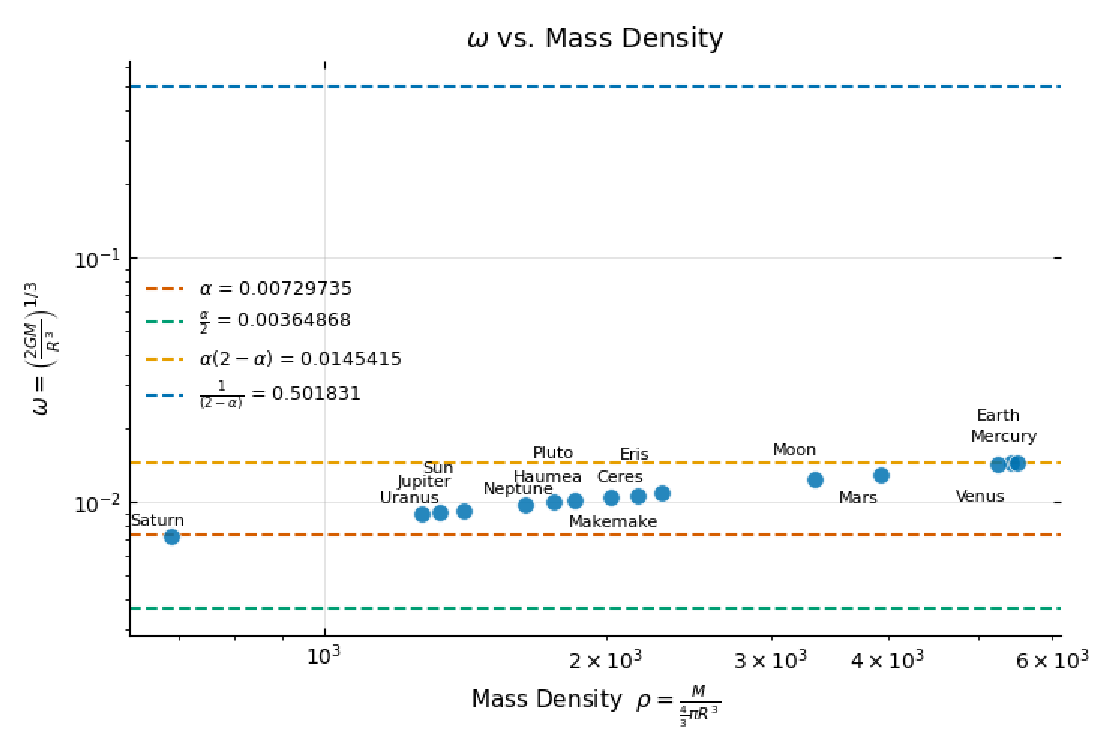
\includegraphics[width=0.9\textwidth]{./diagrams/outputs/omega_mass_density.eps}
\caption{The model quantity $\omega$, identified with $dy$ and constructed from the inverse determinant associated with volume change, plotted as a function of mass density.}\label{fig1}
\label{fig_omega_mass_density}
\end{figure}

We then find through observation that for the least mass dense body in the system, $\Gamma_{\saturn}\left( \sigma \right) \approx 1$.

This gives a set of $3$ equations where the $\Gamma\left( \sigma \right)$ term cancels for the dominant body in the system.

\begin{equation}
    \begin{aligned}
        g_{\oplus} & = R_{\oplus} \left( \frac{\alpha^{3} \left( 2 - \alpha \right)^{3}}{2} \right)  \tau & \pm 0.008\% \\
        g_{\odot} & = R_{\odot} \alpha^{3}  \tau & \pm 1.426\% \\
        g_{\saturn} & = \frac{1}{2} R_{\saturn} \alpha^{3}  \tau & \pm 1.134\% \\
    \end{aligned}
\end{equation}

Which in turn produces a domain where $\alpha \lessapprox \omega \lessapprox \alpha \left( 2 - \alpha \right)$ as shown in figure \ref{fig_omega_mass_density}.

\subsection{Gravitational Parameters}

Due to algebraic symmetries, it's trivial to derive our kinematic velocity through gravitational parameters. What is of interest however, is that we derive what we propose is a more fundamental velocity first. It is only after integrating motion in a manner that is analogous to time that we produce our kinematic velocity. We call this first velocity our \textit{cosmological velocity}, and propose a new geometric interpretation of existing data that may resolve the SNe/CMB velocity discrepancy.


\subsubsection{Cosmological Velocity}

As $\gamma$ is applied as a scalar, we take the average of the integral of $\delta_{\left( M, R \right)}$ to be

\begin{equation}\label{eq_varphi}
    \varphi\left( M, R \right) = \frac{1}{R}\int \delta\left( M, R  \right) = 1 + G \frac{M}{R^{3}}
\end{equation}

Substituting $\varphi\left( M, R \right)$ into equation \ref{eq_v_of_gamma} gives

\begin{equation}\label{eq_v_cosmo}
    \boxed{
    v_{\text{cosmo}} = c \sqrt{1 - \frac{1}{\varphi^2{\left( M, R \right)}}} = 525,493.17 ~ \text{m} / \text{s}
    }
\end{equation}


While this value aligns closely with the correlation carried out by Gordon et al.\cite{gordon_determining_2008}, there remains large uncertainties inherent in SNe observation\cite{Brout2022, Betoule2014}.

\begin{figure}[h]
\centering
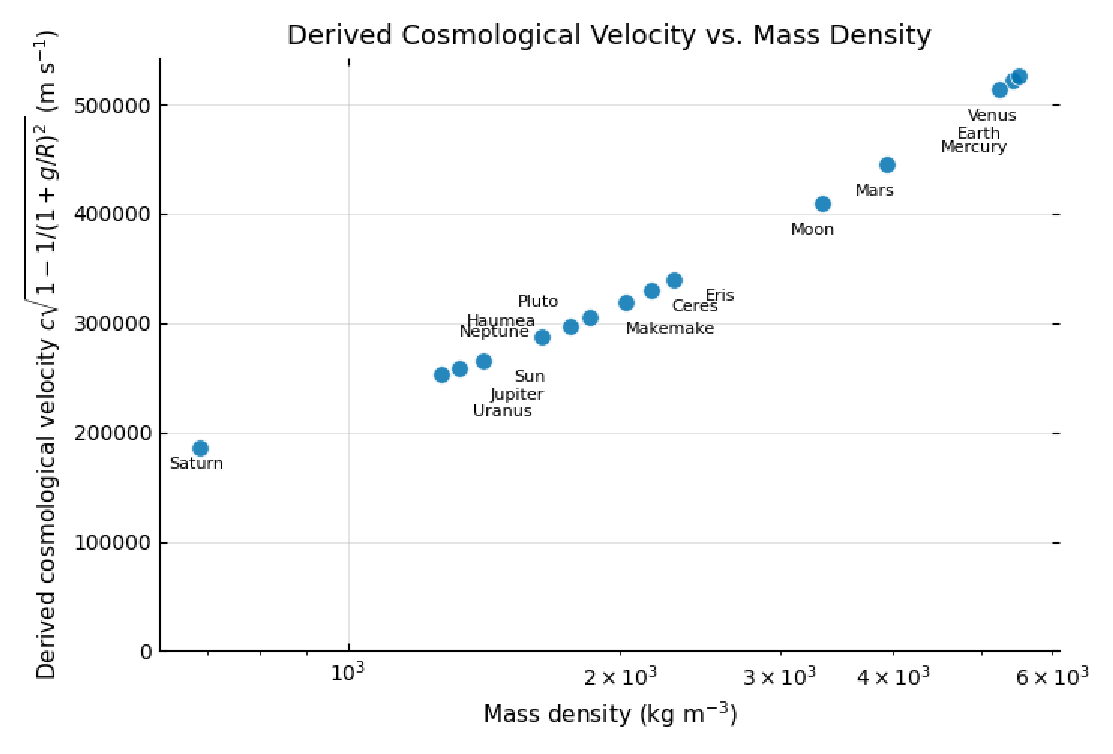
\includegraphics[width=0.9\textwidth]{./diagrams/outputs/cosmo_velocity_mass_density_plot.eps}
\caption{Model-derived cosmological velocity plotted as a function of mass density.}\label{fig1}
\label{fig_mass_density_cosmo_velocity}
\end{figure}

As shown in figure \ref{fig_mass_density_cosmo_velocity}, this function only holds for the theoretical upper bounds of mass density. We speculate that there may exist some yet unknown process in the formation of solar systems, at least at our scale and location within the parent galaxy that leads to a natural function of mass density and velocity. While the details of this process have yet to be resolved, the coordinate transformations described here intrinsically link mass density to velocity as $\vec{g}$ becomes a function of $v$.


\subsubsection{Kinematic Velocity}

We apply the time-equivalent quantity in equation \ref{eq_tau_definition} to equation \ref{eq_varphi}, making equation \ref{eq_varphi} time dependent. Integrating gives

\begin{equation}\label{eq_v_kinematic_1}
\frac{1}{R} \int_0^R \int_0^x \delta \tau~ dR ~ d\tau = 1 + \frac{1}{2} \frac{G M_\oplus}{R^3_\oplus} \left( \frac{\dot{x}}{\hat{x}} \right)^{2}
\end{equation}

We then substitute equation \ref{eq_v_kinematic_1} into equation \ref{eq_v_of_gamma} where $d\tau = 1$

\begin{equation}
    \boxed{
        v_{\scriptsize \text{kinematic}} = c \sqrt{1 - \frac{1}{\left( 1 + \frac{1}{2} G \frac{M}{R^3} \right)^2}} = 371,580 ~ \text{m} / \text{s}
    }
\end{equation}

which matches the 2018 Plank data to within $0.47\%$.

\begin{figure}[h]
\centering
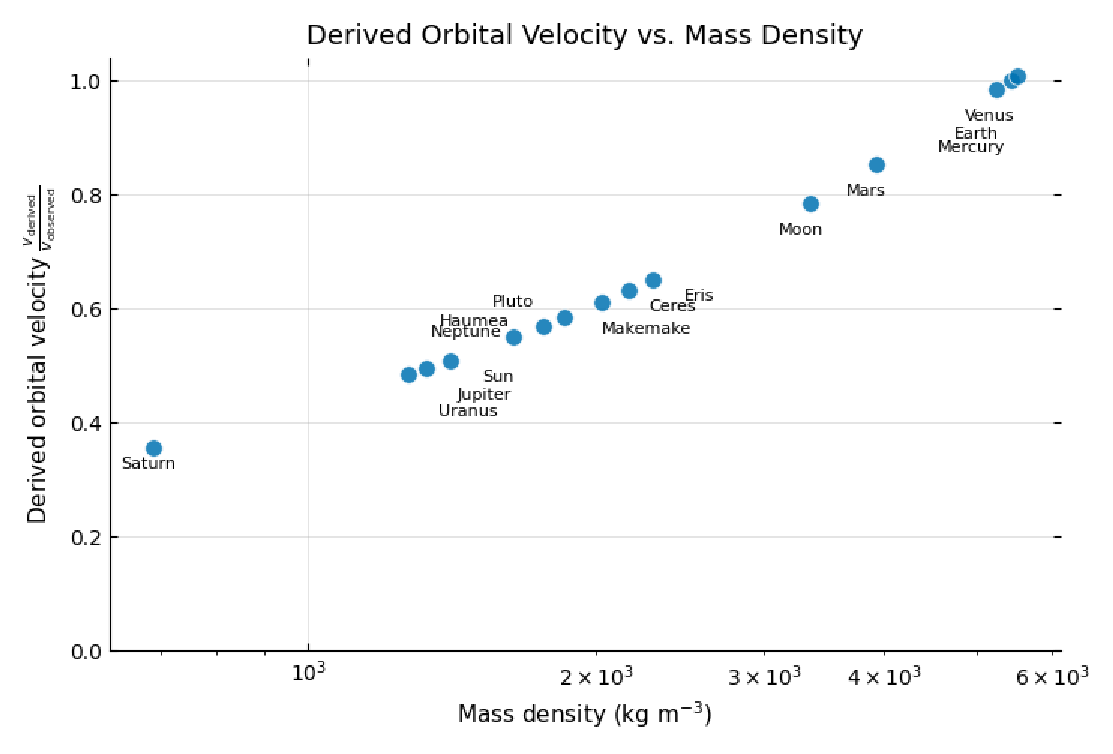
\includegraphics[width=0.9\textwidth]{./diagrams/outputs/mass_density_velocity_plot.eps}
\caption{Model-derived kinematic velocity as a ratio with the velocity found by Eilers et al. plotted as a function of mass density.}
\end{figure}

\subsection{Orbital Velocity}
\begin{figure}[h]
\centering
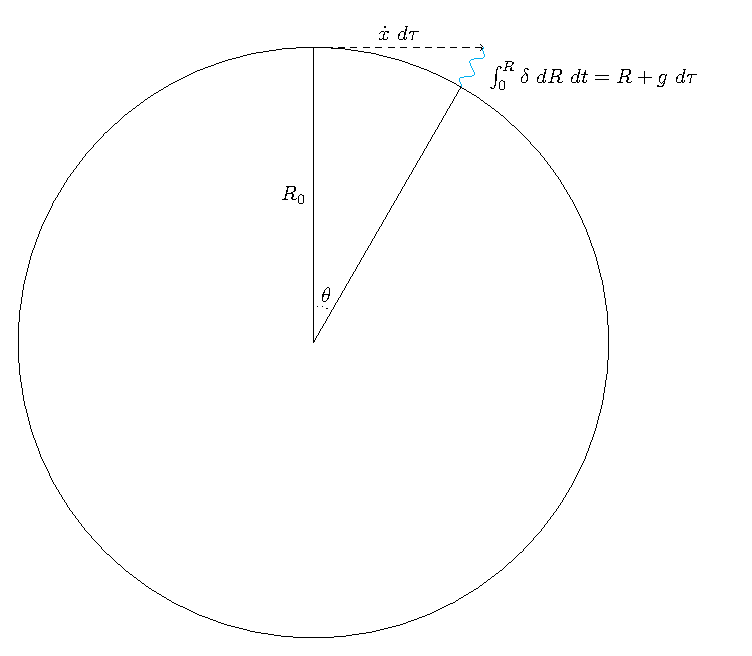
\includegraphics[width=0.5\textwidth]{./diagrams/outputs/trig_orbital_velocity_derivation.eps}
\caption{Geometric construction used in the proposed stable-orbit derivation, showing $R_0$, the angle $\theta$, the displacement $\dot{x}\,d\tau$, and the proposed radial increment $R+g\,d\tau$.}
\label{fig_trig_orbital_velocity}
\end{figure}

\subsubsection{Relativistic Stable Orbit Velocity}

In the simplified single-body system considered here, the spatial dilation described above permits a trigonometric derivation of the stable-orbit velocity as an alternative to the conventional algebraic equality.

Figure \ref{fig_trig_orbital_velocity} represents the geometric construction used in this derivation.

\begin{equation}\label{eq_trig_derivation}
R_0^2 + v_{\text{orbit}}^2 d\tau^2 = \left(\int_0^{R_0} 2 G \frac{M}{R^3}\right)^2 = \left(R_0 + g~ d \tau\right)^2
\end{equation}

Setting $\tau = 1$ gives

\begin{equation}
    \boxed{
    v_{\text{orbit}}\left( M, R \right) = \frac{\sqrt{G M \left(G M + 2 R^{3}\right)}}{R^{2}} 
    }
\end{equation}

For the comparison with the Milky Way, we adopt the enclosed Galactic baryonic mass reported by Cautun et al.~\cite{cautun2020milky}:

\begin{equation}
    M_{\text{enc}} = M_{\mathrm{bar}}(<R_0)
    = 4.44 \times 10^{10}\,M_\odot,
\end{equation}

Here, $R_0 = 8.12\,\mathrm{kpc}$ denotes the Sun's Galactocentric orbital radius\cite{gravity2018detection, bobylev2021estimate}.

For comparison with observation, we use the solar-neighborhood circular velocity reported by Eilers et al.~\cite{Eilers_2019}. Using the adopted enclosed mass and solar orbital radius, the model gives the following orbital velocity:

\begin{equation}\label{eq_orbital_velocity}
    v_{\text{orbit}}\left( M_{\scriptsize\text{enc}}, R_{\scriptsize\text{orbit}} \right) = 216,874 \ \text{m}/ \text{s} = v_{\text{eilers}} \pm 5.59\%
\end{equation}

The model velocity equals the comparison velocity at $M_{\scriptsize \text{enc}} \approx 4.95 \times 10^{10} M_{\odot}$.

The adopted mass scale is also consistent with the characteristic stellar mass scale of approximately $5 \times 10^{10}\,M_\odot$ identified by Yu et al.~\cite{yu2023born} in their FIRE-2 simulations of Milky Way-mass galaxies. Yu et al. associate this scale with a transition in galactic morphology from predominantly disc-dominated to increasingly spheroid-dominated systems. 


\begin{figure}[h]
\centering
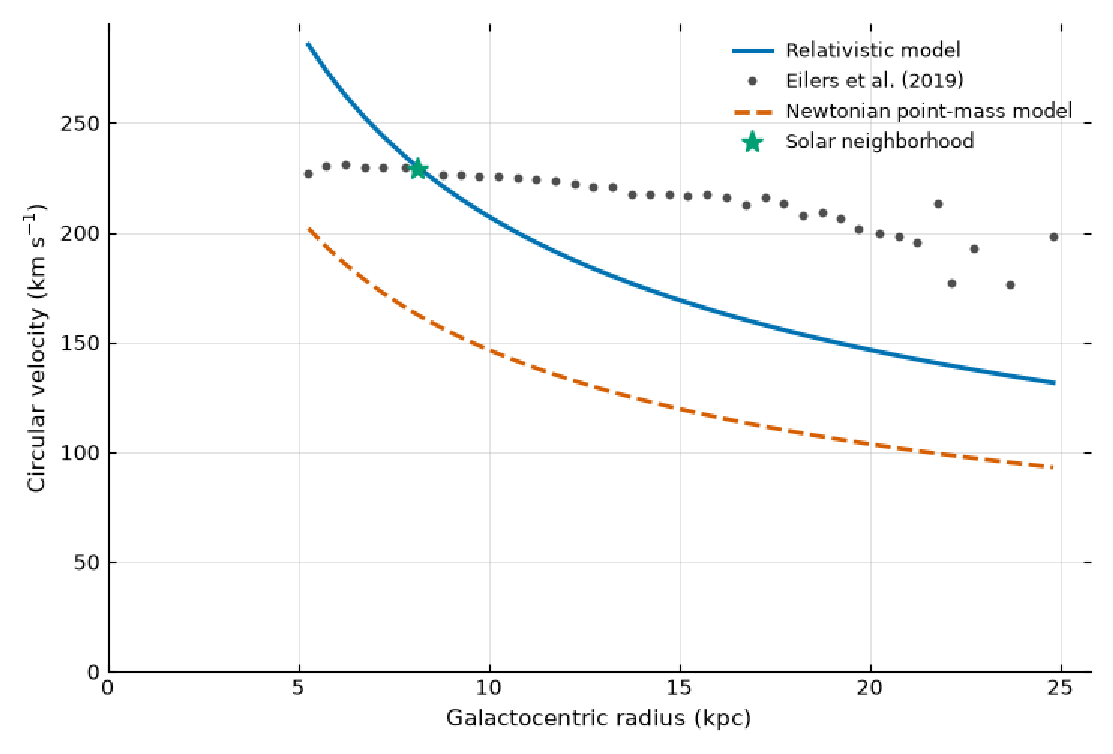
\includegraphics[width=0.9\textwidth]{./diagrams/outputs/eilers_observation.eps}
\caption{Milky Way circular velocity as a function of galactocentric radius. Eilers et al. (2019) measurements are shown as points, alongside the relativistic and Newtonian point-mass model curves. The solar-neighborhood measurement is marked with a star; error bars indicate the reported uncertainties in galactocentric radius and circular velocity.}\label{fig_eilers_observation}
\end{figure}

It is important to note here that $v \left( M, R \right) \approx v_{\text{escape}}$ at $R = R_{\oplus}$ and $M=M_{\oplus}$, not a stable orbit velocity. This discrepency needs to be accounted for by Machian resistance in an n-body system. The associated equations remain elusive, but geometric unity achieved elsewhere appears to indicate the viability of this geometry, such that the sum of this radiating force for all other bodies in the system may induce inertial resistance.

\subsubsection{Kinematic Velocity From Triginometric Orbit Equations}

We now investigate equation \ref{eq_orbital_velocity} by setting 

\begin{equation}
    v_{\text{orbit}} = \sqrt{2 \frac{GM}{R}}
\end{equation}

which is obtained by $E_{\text{kinetic}} = \int g\ dR$. Solving equation \ref{eq_trig_derivation} for $\tau$ and substituting $v_{\text{orbit}}$ gives

\begin{equation}
    \mathrm{d}t = \frac{2 R^{3}}{G M - 2 R^{3}} = -1.000000768
\end{equation}

Inserting this quantity into equation \ref{eq_v_of_gamma} gives

\begin{equation}
    v_{\left( \left|\mathrm{d}t\right| \right)} = 371,580 ~ \text{m} / \text{s}
\end{equation}

which matches the 2018 Plank data to within $0.47\%$.


\subsection{Fifth-Dimensional Spatial Displacement and Gravitational Force}

While most of the derivations to this point have relied on simplified single body solutions, we explore the connections to the KK 5-dimensional metric here. As the KK model imposes a cylindrical condition largely due to the lack of an observable 4th spatial dimension, we derive the magnitude of this 4th dimension from the coordinate transformations described above and apply no such condition.

\subsubsection{Geometric Construction of the Fifth-Dimensional Displacement}

We extend the ordinary three-dimensional displacement into the additional spatial coordinate $y$. Let $dx$ denote the magnitude of the ordinary spatial displacement,

\begin{equation}
    dx = \sqrt{dx_i dx^i},
    \qquad i=1,2,3.
\end{equation}

For spatial velocity magnitude $v$ and displacement parameter $\tau$, as defined in the theoretical framework, the ordinary displacement is

\begin{equation}
    dx = v\tau.
\end{equation}

The proposed construction treats the extended displacement $dx^{(U)}$ as the hypotenuse of a right triangle whose perpendicular components are $dx$ and $dy$ as shown in figure \ref{fig_trig_diagram}. With $\gamma$ denoting the Lorentz factor defined in Equation~\ref{eq_v_of_gamma},

\begin{equation}
    dx^{(U)} = v\tau\gamma.
\end{equation}

Applying the Pythagorean theorem,

\begin{equation}
    \left(dx^{(U)}\right)^2 = dx^2 + dy^2,
\end{equation}

substitution gives

\begin{align}
    dy^2
    &= \left(v\tau\gamma\right)^2-\left(v\tau\right)^2\\
    &= v^2\tau^2\left(\gamma^2-1\right).
\end{align}

Taking the positive magnitude of the additional displacement yields

\begin{equation}
    dy = v\tau\sqrt{\gamma^2-1}
       = \tau\frac{v^2}{\sqrt{c^2-v^2}}.
\end{equation}

The velocity form follows from the Lorentz-factor relation in Equation~\ref{eq_v_of_gamma}.

For constant $v$, differentiation with respect to $\tau$ gives the rate of displacement along $y$:

\begin{equation}
    \boxed{
        \partial_\tau y
        =
        \frac{v^2}{\sqrt{c^2-v^2}}
    }
    \label{eq_dy_dtau}
\end{equation}

\subsubsection{Incorporation into the Kaluza--Klein Metric}

We represent the additional spatial coordinate through the metric component $G_{44}$. For a diagonal five-dimensional metric, the line element is

\begin{equation}
    dS^2
    =
    g_{\mu\nu}dx^\mu dx^\nu
    +
    G_{44}dy^2.
    \label{eq:kk_line_element}
\end{equation}

The corresponding metric tensor has the block structure

\begin{equation}
    \boxed{
    G_{AB}
    =
    \begin{pmatrix}
        g_{\mu\nu} & 0\\
        0 & G_{44}
    \end{pmatrix}
    }
    \label{eq:kk_metric}
\end{equation}

The component $G_{44}$ sets the metric scaling of the additional coordinate. Its radial variation determines the coupling between motion along $y$ and radial motion in the ordinary spatial coordinates.

For radial coordinate $R$, the Christoffel symbol associated with this coupling is

\begin{equation}
    \Gamma^R_{44}
    =
    -\frac{1}{2}g^{RR}
    \frac{\partial G_{44}}{\partial R}.
\end{equation}

For a normalized radial coordinate, $g^{RR}=1$, so

\begin{equation}
    \boxed{
        \Gamma^R_{44}
        =
        -\frac{1}{2}
        \frac{\partial G_{44}}{\partial R}
    }
    \label{eq:radial_christoffel}
\end{equation}

\subsubsection{Finding $G_{44}$}

We take

\begin{equation}
    \partial_x y = \frac{v}{\sqrt{c^{2}  v^{2}}}
\end{equation}

Or

\begin{equation}
    dy = \frac{v}{c^{2} - v^{2}} dx
\end{equation}

We then take the KK line element to be 

\begin{equation}\label{eq_line_element_definition}
    dS^{2} = g_{\mu \nu} dx^{\mu} dx^{\nu} + G_{44}dy^{2}
\end{equation}

and the $\mathbb{R}^{4}$ spatial separation to be

\begin{equation}
    dS^{2}_{\text{spatial}} = dx^{2} + dy^{2}
\end{equation}

where $dx^{2} = dx_i dx^{i}$ for $i = 1, 2, 3$. Expanding this gives

\begin{equation}
    dS^{2}_{\text{spatial}} = dx^{2} \left( 1 + \frac{v^{2}}{c^{2} - v^{2}} \right) = dx^{2} \gamma^{2}
\end{equation}

which matches the expected displacement magnitude of the Lorentz transformations.

Applying a flat metric to the line element defined in equation \ref{eq_line_element_definition} gives

\begin{equation}\label{eq_simple_line_element}
    dS^{2}_{U} = dx^{2} + G_{44} dy^{2}
\end{equation}

yielding

\begin{equation}
    \boxed{
        G_{44}^{\left( U \right)} = 1
    }
\end{equation}

for $dS^{2}_{U} = \gamma^{2} dx^{2}$.

However solving equation \ref{eq_simple_line_element} for $G_{44}$ in the $\mathbf{S}$ coordinate system where $dS^{2}_{S} = d_{i} d^{i}$ gives

\begin{equation}
    \boxed{
        G_{44}^{\left( S \right)} dy^{2} = 0
    }
\end{equation}

indicating that Newtonian mechanics remains contained within a temporal surface, while the relativistic portion of displacement magnitude extends into the 4th spatial dimension, $y$. For this reason, we speculate that inertia has it's origins purely in the relativistic component of displacement; a consequence of a Machian-like resistance along the 4th dimension.

\section{Discussion}

\subsection{The Appearance of Electromagnetic Parameters}

We do not claim to derive a direct mechanical derivation for the fine structure constant, nor an explanation for it's appearance in section \ref{sec_equivalence_principle}. We simply apply the coordinate transformations defined in section \ref{sec_theoretical_framework} and discover that $\alpha$ appears repeatedly. While the probability is difficult to quantize, we feel that this repeated appearance of $\alpha$, appearing in gravitational approximations for all 3 of the local bodies with boundary like characteristics likely indicates a shared function which itself contains or produces $\alpha$. Due to the hypersphere-like geometry that arises from this model, we propose further investigation into the boundary between Wyler's derivation\cite{Wyler1969} of $\alpha$ and the $4 + 0$ space-time described here.


%%===========================================================================================%%
%% If you are submitting to one of the Nature Portfolio journals, using the eJP submission   %%
%% system, please include the references within the manuscript file itself. You may do this  %%
%% by copying the reference list from your .bbl file, paste it into the main manuscript .tex %%
%% file, and delete the associated \verb+\bibliography+ commands.                            %%
%%===========================================================================================%%

\bibliography{citations.bib}% common bib file
%% if required, the content of .bbl file can be included here once bbl is generated
%%\input sn-article.bbl

\end{document}
